\documentclass{article}
\def\npart {2}
\def\nterm {LMS Summer School}
\def\nyear {2020}
\def\nlecturer {Professor Sarah Whitehouse - University of Sheffield}
\def\ncourse {Combinatorics of Young tableaux and symmetric groups}

\input{header}

\begin{document}
  \maketitle
\ytableausetup{centertableaux}

\section{Overview}

\begin{itemize}
  \item Basic reminders about groups
  \item Definitions of partitions, Young Diagrams and tableaux.
  \item How many standard tableaux are there?
  \item There are two answers; the hook formula and the determinant formula.
  \item Some ideas of the proof - prove the two formulas give the same answer. More detail about the hook formula, via a bijective proof.
  \item Sketch of the relevance to representations of the symmetric group.
\end{itemize}

Useful resource - Bruce E. Sagan, \textit{The Symmetric Group: Representations, Combinatorial Algorithms and Symmetric Functions}

\subsection{Symmetric Group and Permutations}
Let $n \in \N$,

\begin{ndefi}{Symmetric Group}
  The $n^{th}$ symmetric group is $S_n$, and it's the group of all bijections from $\{1, 2, \dots, n\}$ to itself.
\end{ndefi}

Permutations are multiplied from right to left as that's the convention for function composition.\\
There are several standard ways to write perms,
The same permutations $\sigma$ in $S_7$, two line notation,
$$ \begin{matrix}
  1 & 2 & 3 & 4 & 5 & 6 & 7 \\
  6 & 2 & 5 & 7 & 3 & 4 & 1
\end{matrix} $$
and one line notation,
$$ \begin{matrix}
  6 & 2 & 5 & 7 & 3 & 4 & 1
\end{matrix} $$
and in cycle notation,
$ (1 6 4 7)(3 5)(2) $ or $ (1 6 4 7)(3 5) $
this means that $1 \to 6 \to 4 \to 7 \to 1 \dots$ and $3 \to 5 \to 3 \to \dots$ and $2$ maps to itself. The two doesn't necessarily need to be written as it may be seen as redundant.\\

The composition of $\pi\sigma$ where $\sigma = (1 6 4 7)(3 5)(2) $ and $\pi = (1 4)$, then,
$$ \pi\sigma = (1 4)(1 6 4 7)(3 5) = (1 6)(3 5)(4 7) $$
this isn't very efficient as there are things written more than once. Read right to left, and just work through it and write it down.

\begin{ndefi}{k-cycle}
  A $K$-cycle is a cycle containing k elements
\end{ndefi}
The cycle type of a permutation is an expression of the form $(1^{m_1}, 2^{m_2}, \dots, n^{m_n})$ where $M_k$ is the number of k-cycles.\\
For example, $\sigma$ has cycle type, $(1^1, 2^1, 3^0, 4^1, 5^0, 6^0, 7^0)$.\\

\begin{ndefi}{Conjugation}
  In Group Theory, take a group $G$, the elements $g$ and $h$ are conjugate if the exists some $k\in G$, st, $g = khk^{-1}$.
\end{ndefi}
Conjugacity is an equivalence relation, so the group splits up into non-intersecting conjugacy classes.\\
\begin{ndefi}{Conjugacy Class}
  The set of all elements conjugate to $g \in G$ is called the conjugacy class of $g$.
\end{ndefi}

\subparagraph{Conjugacy Classes and Cycle Types}
\begin{remark}
  For the inverse, write down each of the elements in reverse order.
\end{remark}

If,
$$ \pi = (i_1, i_2, \dots, i_l)\dots (i_r, i_{r+1}, \dots, i_n) \in S_n $$
then,
$$ \sigma\pi\sigma^{-1} = (\sigma(i_1), \sigma(i_2), \dots, \sigma(i_l))\dots (\sigma(i_r), \sigma(i_{r+1}), \dots, \sigma(i_n)) $$
You have the same cycle type, you just `apply' $\sigma$. Same cycle type and the number replaced with what you are conjugating by. For example, $\pi = (1 4)$ (2 cycle, transposition) and $\sigma = (1 6 4 7)(3 5)$ as before, $\sigma \pi \sigma^{-1} = (6 7) $. It follows that,
\begin{nlemma}
  Two permutations are conjugate if and only if they have the same cycle type.
\end{nlemma}
We haven't only done one side as if we take a $\sigma$, we can just take an appropriate $\pi$.\\

Conjugacy is very important in group theory, they are used in classification results and philoe theorems. A group acts on itself by conjugation, it acts by conjugation of that group action. You have orbits and stabilizers and you can deduce things about the structure of the group. There are irreducible representations and there is each one for each conjugacy class of the group.

\section{Paritions and Young Tableaux}

\begin{ndefi}{\textit{Partition}}
  A partition of $n$ is a finite sequence of natural numbers $\l = (\l_1, \l_2, \dots, \l_r)$ where $\l_i \ge \l_{i+1}$ for all $i$ and $\sum_{i=1}^r \l_i = n$. We write $(\l_1, \l_2, \dots, \l_r) \vdash n$ this to mean partition,
\end{ndefi}

For example, $(5, 3, 1) \vdash 9$. We represent paritions by diagrams, in the form of left justified arrays of boxes. For the partition $(\l_1, \l_2, \dots, \l_r)$, we draw $\l_1$ on the top, then $\l_2$, and so on. Let us take $(5, 3, 1)$.

We saw earlier that two elements of $S_n$ are in the same conjugacy class if and only if they have the same cycle type.\\
We can equivilent record a cycle by a partition of $n$. For our previous example, $\s = (1 6 4 7)(3 5)(2)$ and record the cycle type as $(4, 2, 1)$, as per our pervious definition. This means that there are a bijection between partitions of $n$ \\

\begin{ndefi}
  A Young Tableau of shape $\l$, where $\l \vdash n$, is a bijective assignment of the numbers $1, 2, \dots, n$  to the boxes of the diagram of $\l$.
\end{ndefi}
Clearly, the number of such tableaux is $n!$. Such a tableaux is called standard if each column and row is increasing.\\
First we fix $n$, then draw the diagram and then assign $1$ up to $n$ into the boxes with constraints of increasing in each row and column. We will write $f^\l$ as the number of standard young tableaux of shape $\l$. Understanding the number of $f^\l$ and our importance will be our focus.

\subsection{Alfred Young}
Reverend Alphred Young, came up with the tableaux. ``The original man of the year, who would have ranked a higher place in the list had he directed his attention to the examination schedule''. He attaned a 2:2 from Cambridge.

\subsection{Tableaux}
We are going to consider $S_3$. Here are the 6 young tableaux of shape $(2, 1)$.
\begin{figure}[!ht]
  \centering
  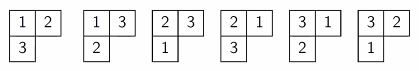
\includegraphics{./figures/L1.1}
  \caption{The Young Tableaux for $(2, 1)$.}
  \label{}
\end{figure}
% write out each of the diagrams.
The first two are standard tableaux and the rest are not. The conclusion is that $f^{(2, 1)} = 2$.




\end{document}
